\documentclass[11pt]{amsart}
\usepackage[margin=1.1in]{geometry}
\usepackage{amssymb,mathtools}
\usepackage{graphicx}
\usepackage{booktabs}
\usepackage{tikz}
\usetikzlibrary{arrows.meta,positioning}
\usepackage{xurl}
\usepackage[colorlinks=false,hidelinks]{hyperref}
\numberwithin{equation}{section}
\theoremstyle{plain}
\newtheorem{thm}{Theorem}[section]
\newtheorem{lem}[thm]{Lemma}
\newtheorem{prop}[thm]{Proposition}
\newtheorem{cor}[thm]{Corollary}
\theoremstyle{definition}
\newtheorem{defn}[thm]{Definition}
\theoremstyle{remark}
\newtheorem{rem}[thm]{Remark}
\newcommand{\Z}{\mathbb{Z}}
\newcommand{\Q}{\mathbb{Q}}
\newcommand{\R}{\mathbb{R}}
\newcommand{\C}{\mathbb{C}}
\newcommand{\cA}{\mathcal{A}}
\newcommand{\cE}{\mathcal{E}}
\newcommand{\cL}{\mathcal{L}}
\newcommand{\e}{\mathbf{e}}
\newcommand{\pmi}{\phi_{-2,1}}
\newcommand{\pz}{\phi_{0,1}}
\newcommand{\tPhi}{\widetilde{\Phi}}
\newcommand{\sm}[4]{\left(\begin{smallmatrix}#1&#2\\#3&#4\end{smallmatrix}\right)}

\title[Positive Indices for All Charges in CHL Models]{Positive Single-Centred Black Hole Indices for All Charges in the $\mathbb Z_3$, $\mathbb Z_5$ and $\mathbb Z_7$ CHL Models}
\author{Deep Bhattacharjee}
\address{Formerly, Electro-Gravitational Space Propulsion Laboratory (EGSPL), Bhubaneswar, Odisha 751030, India; formerly, University of Calcutta (Heramba Chandra College), 23/49 Gariahat Road, Golpark, Kolkata 700029, West Bengal, India}
\email{d.bhattacharjee@erl-forschung.de}
\subjclass[2020]{11F50 (primary); 11F30, 11F37, 81T30, 83E30}
\keywords{CHL models, single-centred black holes, Rademacher expansion}
\newcommand{\ERRthree}{$4.9\cdot10^{-22}$}\newcommand{\ERRfive}{$6.1\cdot10^{-9}$}\newcommand{\ERRseven}{$3.0\cdot10^{-8}$}
\newcommand{\UthreeA}{$7.8\cdot10^{-10}$}\newcommand{\UthreeB}{$2.1\cdot10^{-72}$}\newcommand{\UfiveA}{$1.3\cdot10^{-9}$}\newcommand{\UfiveB}{$3.9\cdot10^{-31}$}\newcommand{\UsevenA}{$1.4\cdot10^{-9}$}\newcommand{\UsevenB}{$5.1\cdot10^{-15}$}
\newcommand{\CNthree}{$2{,}090{,}978$}\newcommand{\CNfive}{$4{,}968{,}027$}\newcommand{\CNseven}{$4{,}400{,}496$}\newcommand{\CMthree}{$0.2057$ at $(400,400,400)$}\newcommand{\CMfive}{$0.1993$ at $(400,560,400)$}\newcommand{\CMseven}{$0.1651$ at $(399,399,285)$}
\newcommand{\LGthree}{$0.203$}\newcommand{\LGfive}{$0.165$}\newcommand{\LGseven}{$0.078$}

\begin{document}
\begin{abstract}
In the $\Z_3$, $\Z_5$ and $\Z_7$ CHL models of four-dimensional $\mathcal N=4$ string theory, the index of every single-centred quarter-BPS black hole is positive, as Sen predicted. The proof combines a level-$N$ Rademacher expansion of the relevant mock Jacobi forms, a resummation of its dominant terms into the square of an eta quotient, and certified bounds for everything else.
\end{abstract}
\maketitle

%%==================================================================
\section{Introduction}
%%==================================================================

A quarter-BPS dyon in an $\mathcal N=4$ string theory in four dimensions carries an electric charge $Q$ and a magnetic charge $P$. When the charges admit a single-centred black hole, its microstates carry zero angular momentum after the fermion zero modes of the broken supersymmetries are removed, and the black hole contributes a positive amount to the helicity trace index. Sen turned this into a prediction about Fourier coefficients of Siegel modular forms \cite{Sen11}: the single-centred index $d_*(Q,P)$, extracted from the inverse of the dyon partition function on the attractor contour, is positive.\footnote{The argument is physical. The near-horizon geometry of a single-centred black hole has an $SU(2)$ rotation symmetry, so the states counted by the index all have $J_3=0$, and then the sign $(-1)^{2J_3}$ in the helicity trace is $+1$ for every state. Sen checked the sign numerically for many charges of heterotic string theory on $T^6$ and of the CHL models of orders $2,3,5,7$ \cite{Sen11}; the entropy function and attractor background behind the statement are reviewed in \cite{Sen08}.}

For type~II string theory on $K3\times T^2$, where the partition function is the inverse of the Igusa cusp form \cite{DVV97}, the prediction is a theorem: Bringmann and Murthy treated the two smallest magnetic charges \cite{BM13}, and Rossell\'o all charges \cite{Ros24}. The CHL models \cite{CHL95} are $\Z_N$ orbifolds whose partition functions $\tPhi_k$ are Siegel modular forms for congruence subgroups \cite{JS06,DJS06}. Bhand, Sen and Singh showed that the Fourier--Jacobi coefficients of $1/\tPhi_k$ are meromorphic Jacobi forms whose finite parts are mock Jacobi forms, and that on an explicit set of charges $d_*$ is a Fourier coefficient of such a finite part \cite{BSS25}; a generating function for $d_*$ in general $\Z_N$ CHL models was constructed in \cite{Sin26}. The conjecture is proved for every charge of the $\Z_2$ model in \cite{Bha26a}, for the toroidal compactifications and the heterotic string under stated arithmetic conditions in \cite{Bha26b}, and for the first row $Q^2=2/N$ of the $\Z_3$, $\Z_5$ and $\Z_7$ models in \cite{Bha26c}.

This paper completes the three models of odd prime order. For $N\in\{3,5,7\}$ we put $k+2=24/(N+1)$, so $k=4,2,1$, and normalise the charges as
\begin{equation}\label{eq:charges}
m=\tfrac N2Q^2,\qquad n=\tfrac12P^2,\qquad \ell=Q\cdot P,\qquad D=Q^2P^2-(Q\cdot P)^2=\frac{4mn}{N}-\ell^2 .
\end{equation}

\begin{thm}\label{thm:main}
Let $N\in\{3,5,7\}$. In the $\Z_N$ CHL model, $d_*(Q,P)>0$ for every pair of charges with $Q^2>0$, $P^2>0$ and $D>0$.
\end{thm}

The proof follows the plan of \cite{Bha26a}, and Figure~\ref{fig:map} shows it. Dualities reduce every charge to one with $m\le n$, $0\le\ell\le m$ and $x:=\sqrt D/m\ge\sqrt3/N$, for which $d_*$ is a Fourier coefficient of a finite part (Section~\ref{sec:red}). For such a charge an exact expansion of Rademacher type writes $d_*$ as a positive factor $\cE$ times $\cL+R$ (Section~\ref{sec:exp}), where $\cL$ collects the terms of one family of walls and $R$ the rest. As $m$ grows, $\cL$ tends to
\begin{equation}\label{eq:PN}
|P_N(z)|^2,\qquad P_N(z)=\prod_{j\ge1}(1-z^j)^{-(k+2)}(1-z^{Nj})^{-(k+2)},\qquad z=e^{-\pi x+\pi i\ell/m},
\end{equation}
which never vanishes, and whose minimum over the reduced charges is $0.205$, $0.199$ and $0.165$ for $N=3,5,7$ (Section~\ref{sec:lead}). The rest of the paper shows that $\cL+R$ stays positive for every reduced charge. There are three regimes.

\begin{itemize}
\item Away from the corner where $x$ is close to $\sqrt3/N$ (precisely, for $x\ge x_1$ with $x_1=1,0.8,0.6$), each term of $\cL-|P_N|^2$ and of $R$ is bounded separately, by explicit inequalities for Bessel functions (Section~\ref{sec:away}).
\item In the corner, the terms of $\cL$ cancel against each other, and bounding them one at a time overshoots by a factor of about a thousand. For $Q^2<600/N$ we evaluate $\cL$ for each corner charge separately, with rigorous bounds for the omitted terms (Section~\ref{sec:corner}).
\item For $Q^2\ge600/N$ we expand $\cL$ in powers of $1/m$ to tenth order, bound the remainder by interval arithmetic, and check the resulting function of $(x,\ell/m)$ on a certified grid (Section~\ref{sec:large}).
\end{itemize}
The finitely many charges with small discriminant are settled by computing $d_*$ exactly from the product formula (Section~\ref{sec:exact}), and Section~\ref{sec:proof} assembles the proof. All programs are public.

\begin{figure}[t]
\centering
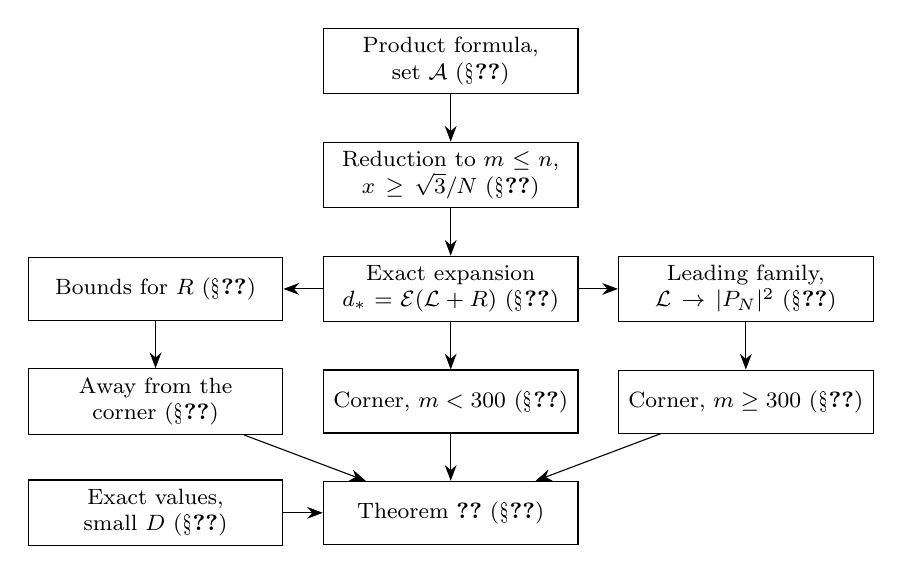
\begin{tikzpicture}[node distance=6mm and 5mm, every node/.style={draw, rectangle, align=center, font=\footnotesize, minimum height=8mm, text width=30mm}, >={Stealth[length=2mm]}]
\node (pf) {Product formula, set $\cA$ (\S\ref{sec:pf})};
\node (red) [below=of pf] {Reduction to $m\le n$, $x\ge\sqrt3/N$ (\S\ref{sec:red})};
\node (exp) [below=of red] {Exact expansion $d_*=\cE(\cL+R)$ (\S\ref{sec:exp})};
\node (lead) [right=of exp] {Leading family, $\cL\to|P_N|^2$ (\S\ref{sec:lead})};
\node (err) [left=of exp] {Bounds for $R$ (\S\ref{sec:err})};
\node (aw) [below=of err] {Away from the corner (\S\ref{sec:away})};
\node (co) [below=of exp] {Corner, $m<300$ (\S\ref{sec:corner})};
\node (lg) [below=of lead] {Corner, $m\ge300$ (\S\ref{sec:large})};
\node (mt) [below=of co] {Theorem~\ref{thm:main} (\S\ref{sec:proof})};
\node (ex) [left=of mt] {Exact values, small $D$ (\S\ref{sec:exact})};
\draw[->] (pf) -- (red); \draw[->] (red) -- (exp); \draw[->] (exp) -- (co); \draw[->] (lead) -- (lg);
\draw[->] (err) -- (aw); \draw[->] (exp) -- (err); \draw[->] (exp) -- (lead);
\draw[->] (aw) -- (mt); \draw[->] (co) -- (mt); \draw[->] (lg) -- (mt); \draw[->] (ex) -- (mt);
\end{tikzpicture}
\caption{The structure of the proof. An arrow means that the section at its tail is used in the section at its head.}
\label{fig:map}
\end{figure}

%%==================================================================
\section{The Partition Function and the Single-Centred Index}\label{sec:pf}
%%==================================================================

We recall the set-up of \cite{Bha26c}, to which we refer for proofs. Write $\e(t)=e^{2\pi it}$, let $\pmi$ and $\pz$ be the weak Jacobi forms of weight $-2$ and $0$ and index one \cite[\S9]{EZ85}, and let
\[
E_N(\tau)=\frac{NE_2(N\tau)-E_2(\tau)}{N-1}=1+\frac{24}{N-1}\sum_{n\ge1}\sigma^{(N)}(n)q^n,\qquad \sigma^{(N)}(n)=\sum_{d\mid n,\ N\nmid d}d .
\]
The twisted elliptic genera of $K3$ for a symplectic automorphism of prime order $N$ are \cite{JS06,DJS06}
\begin{equation}\label{eq:genera}
\begin{gathered}
F^{(0,0)}=\tfrac{2}{N}\pz,\qquad F^{(0,s)}=\tfrac{2}{N(N+1)}\pz+\tfrac{2}{N+1}\pmi E_N(\tau),\\
F^{(r,rt)}=\tfrac{2}{N(N+1)}\pz-\tfrac{2}{N(N+1)}\pmi E_N\!\left(\tfrac{\tau+t}{N}\right),
\end{gathered}
\end{equation}
for $1\le s\le N-1$, $1\le r\le N-1$ and $t\in\Z/N$. Write $F^{(r,s)}=\sum_{b\in\{0,1\}}\sum_{j\equiv b\,(2)}\sum_{n}c_b^{(r,s)}(4n-j^2)q^n\zeta^j$. The partition function is \cite{DJS06}
\begin{equation}\label{eq:product}
\tPhi_k(\rho,\sigma,v)=\e\!\left(\rho+\tfrac{\sigma}{N}+v\right)\prod_{\substack{\kappa,l\in\Z_{\ge0},\ j\in\Z\\ j<0\text{ if }\kappa=l=0}}\bigl(1-\e(\tfrac{\kappa}{N}\sigma+l\rho+jv)\bigr)^{E(\kappa,l,j)},
\end{equation}
with $E(\kappa,l,j)=\sum_{s=0}^{N-1}\e(-sl/N)\,c_b^{(r,s)}(4\kappa l/N-j^2)$, $r\equiv\kappa\pmod N$, $b\equiv j\pmod2$. Put $x=\e(\sigma/N)$, $y=\e(v)$, $p=\e(\sigma)$. Expanding $1/\tPhi_k=\sum_{m\ge-1}\varphi_m(\sigma,v)\e(m\rho)$, each $\varphi_m$ with $m\ge1$ is a meromorphic Jacobi form of weight $-k$ and index $m$ with double poles at $v\in\Z\sigma+\Z$ \cite[Theorem~5.2]{BSS25}, and its polar part is \cite[(5.45)]{BSS25}
\begin{equation}\label{eq:polar}
\varphi^P_m=\frac{d(m)}{g(\sigma/N)}\sum_{s\in\Z}\frac{p^{ms^2+s}y^{2ms+1}}{(1-p^sy)^2},\qquad g(\tau)=\eta(\tau)^{k+2}\eta(N\tau)^{k+2},
\end{equation}
where $d(a)$ denotes the coefficient of $q^a$ in $1/g(\tau)=\sum_{a\ge-1}d(a)q^a$. Since $(k+2)(N+1)=24$, $1/g=q^{-1}P_N(q)$, so $d(a)$ is the coefficient of $q^{a+1}$ in \eqref{eq:PN} and is a positive integer for $a\ge-1$. The finite part $\varphi^F_m=\varphi_m-\varphi^P_m=\sum c^F_m(n,\ell)x^ny^\ell$ is a mock Jacobi form. Let $\cA$ be the set of charges with $m,n>0$, $D>0$ and
\begin{equation}\label{eq:setA}
\min_{\substack{m_1\in N\Z,\ s\in\Z\\ m_1\mid s(s+1)}}\Bigl[(m_1\ell+2ms+m)^2+m_1^2D\Bigr]\ \ge\ m^2 .
\end{equation}
By \cite[Theorem~5.4(a) and (5.57)]{BSS25}, for every charge in $\cA$,
\begin{equation}\label{eq:dstar}
d_*(Q,P)=(-1)^{\ell+1}c^F_m(n,\ell).
\end{equation}

\begin{lem}\label{lem:E}
$E(\kappa,l,j)$ depends only on $4\kappa l/N-j^2$, on $j\bmod 2$, and on the unordered pair $\{[N\mid\kappa],[N\mid l]\}$. In particular $E(\kappa,l,j)=E(l,\kappa,j)$.
\end{lem}

\begin{proof}
Write $c_{01}$, $h$ and $\tilde h$ for the coefficients, at the discriminant $\Delta=4\kappa l/N-j^2$ and parity $b$, of $\pz$, of $\pmi E_N(\tau)$ and of $\pmi E_N(\tau/N)$, where the $q$-exponent is $\kappa l/N$; $c_{01}$ and $h$ vanish unless this exponent is an integer. Put $a_N=2/(N(N+1))$.

If $N\mid\kappa$, then $r=0$, and \eqref{eq:genera} gives $E=\frac2Nc_{01}+\bigl(\sum_{s\ne0}\e(-sl/N)\bigr)\bigl(a_Nc_{01}+\frac{2}{N+1}h\bigr)$. The sum over $s$ is $N-1$ if $N\mid l$ and $-1$ otherwise, so $E=\frac2Nc_{01}+(N-1)(a_Nc_{01}+\frac2{N+1}h)$ if $N\mid l$, and $E=\frac{2}{N+1}(c_{01}-h)$ if $N\nmid l$.

If $N\nmid\kappa$, only the sectors $s=rt$ contribute. The coefficient of $q^{\kappa l/N}$ in $\pmi E_N((\tau+t)/N)$ is $\e(t\kappa l/N)\tilde h$, and $\sum_t\e(-rtl/N)\e(t\kappa l/N)=N$ because $r\equiv\kappa$. So $E=N a_N(c_{01}-\tilde h)=\frac{2}{N+1}(c_{01}-\tilde h)$.

Each value depends only on $\Delta$, $b$ and the two divisibilities. The two mixed cases agree: if $N\nmid\kappa$ and $N\mid l$, the exponent $\kappa l/N$ is an integer, and the integral powers of $q$ in $E_N(\tau/N)$ form $E_N(\tau)$, because $\sigma^{(N)}(Nn)=\sigma^{(N)}(n)$.\footnote{A divisor of $Nn$ that is not divisible by $N$ divides $n$, since $N$ is prime. So the coefficient of $q^{n}$ in $E_N(\tau/N)$, which is the coefficient of $q^{Nn}$ in $E_N(\tau)$, equals the coefficient of $q^n$ in $E_N(\tau)$.} Hence $\tilde h=h$ and $E=\frac{2}{N+1}(c_{01}-h)$, the value for $N\mid\kappa$, $N\nmid l$. We have also confirmed the symmetry $E(\kappa,l,j)=E(l,\kappa,j)$ numerically for all $\kappa,l\le24$, $|j|\le12$.
\end{proof}

%%==================================================================
\section{Dualities and Reduced Charges}\label{sec:red}
%%==================================================================

\subsection{Two symmetries}
The group $\Gamma_0(N)$ acts on charge vectors by
\begin{equation}\label{eq:action}
\sm abcd\cdot(m,n,\ell)=\Bigl(a^2m+Nab\ell+Nb^2n,\ \tfrac{c^2}{N}m+cd\ell+d^2n,\ \tfrac{2ac}{N}m+(ad+bc)\ell+2bdn\Bigr),
\end{equation}
which preserves $D$ and is the action of the S-duality transformations $Q\mapsto aQ+bP$, $P\mapsto cQ+dP$ in the normalisation \eqref{eq:charges}. The S-duality group of the $\Z_N$ CHL model is $\Gamma_1(N)$ \cite{JS06}, and $d_*$ is invariant under it, because the attractor contour moves with the charges \cite{Sen08,BSS25}.

\begin{prop}\label{prop:sym}
Let $N\in\{3,5,7\}$. The coefficients of $1/\tPhi_k$ satisfy $c(m,n,\ell)=c(n,m,\ell)$, where $c(m,n,\ell)$ is the coefficient of $\e(m\rho)x^ny^\ell$ in a given chamber and its image under $(\rho,\sigma)\mapsto(\sigma/N,N\rho)$. Moreover $d_*$ is invariant under $\Gamma_0(N)$ and under $(m,n,\ell)\mapsto(n,m,\ell)$.
\end{prop}

\begin{proof}
By Lemma~\ref{lem:E} the product \eqref{eq:product} is invariant under $\kappa\leftrightarrow l$, and its prefactor $\e(\rho+\sigma/N+v)$ is invariant under $\rho\leftrightarrow\sigma/N$. So $\tPhi_k(\rho,\sigma,v)=\tPhi_k(\sigma/N,N\rho,v)$, which exchanges $m$ and $n$. For $\Gamma_0(N)$: the action \eqref{eq:action} on the exponent vectors $(\kappa,l,j)$ preserves $4\kappa l/N-j^2$, the parity of $j$, and the conditions $N\mid\kappa$ and $N\mid l$, since $a$ and $d$ are prime to $N$ and $\kappa'\equiv a^2\kappa$, $l'\equiv d^2l\pmod N$. By Lemma~\ref{lem:E} it therefore preserves the exponents. The product \eqref{eq:product} is the Borcherds lift of the vector-valued form built from the $F^{(r,s)}$, and an isometry of the lattice that preserves the input preserves the lift up to a character \cite[Theorem~13.3]{Bor98}; together with the Weyl vector, which is fixed, this shows that $\tPhi_k$ is modular under the image of $\Gamma_0(N)$. The single-centred index is then invariant, because both its definition through the attractor contour and the chamber structure are covariant. We have also checked the invariance directly: for every charge in $\cA$ with $m\le5$ and $n\le57$ whose image under a generator of $\Gamma_0(N)/\{\pm1\}\Gamma_1(N)$, reduced back by $\Gamma_1(N)$, also lies in this box, the two values of $d_*$ computed from \eqref{eq:product} agree exactly ($1120$, $9$ and $12$ pairs for $N=3,5,7$).
\end{proof}

We define $d_*$ on every charge with $D>0$ through its value at any representative in $\cA$ of its orbit under the group generated by $\Gamma_0(N)$ and the exchange; Proposition~\ref{prop:sym} shows that this is consistent, and Lemma~\ref{lem:redA} below that a representative exists.

\subsection{Reduced charges}
Put $q(a,b)=a^2m+Nab\ell+Nb^2n$, the first entry of \eqref{eq:action}, and
\[
w=\frac{N(\ell+i\sqrt D)}{2m},\qquad\text{so that}\qquad q(a,b)=m\,|a+bw|^2 .
\]
\begin{defn}
A charge $(m,n,\ell)$ with $D>0$ is \emph{reduced} if $m\le n$, $0\le\ell\le m$ and $q(a,b)\ge m$ for all coprime $(a,b)$ with $b\ne0$ and $N\nmid a$.
\end{defn}

\begin{lem}\label{lem:redA}
Every orbit contains a reduced charge, and every reduced charge lies in $\cA$.
\end{lem}

\begin{proof}
The first rows of matrices in $\Gamma_0(N)$ are the coprime pairs $(a,b)$ with $N\nmid a$, and $q$ is positive definite, so the values $q(a,b)$ have a minimum; take a matrix realising it. The matrix $\sm10{N}1$ and its powers fix $m$ and shift $\ell$ by multiples of $2m$, and $-1$ and the exchange are available, so we may arrange $|\ell|\le m$, then $\ell\ge0$ (by $(a,b,c,d)=(1,0,0,-1)$ composed with the exchange, which maps $\ell\mapsto-\ell$), and $m\le n$ (if $n<m$ the exchange lowers $m$). For the second statement, write the bracket in \eqref{eq:setA} as $|m_1(\ell+i\sqrt D)+m(2s+1)|^2=m^2|(2s+1)+2bw|^2$ with $m_1=Nb$. If $b=0$ the bracket is $m^2(2s+1)^2\ge m^2$. If $b\ne0$, then $N\mid s(s+1)$, so $2s+1\equiv\pm1\pmod N$; let $g=\gcd(2s+1,2b)=\gcd(2s+1,b)$. Then $(a',b')=((2s+1)/g,2b/g)$ is coprime with $N\nmid a'$ and $b'\ne0$, so $|(2s+1)+2bw|=g|a'+b'w|\ge g\ge1$ by reducedness.
\end{proof}

\begin{lem}\label{lem:xmin}
For a reduced charge, $x=\sqrt D/m\ge\sqrt3/N$.
\end{lem}

\begin{proof}
We have $\operatorname{Re}w=N\ell/(2m)\in[0,N/2]$ and $\operatorname{Im}w=Nx/2$. If $\operatorname{Re}w\ge1/2$, the integer $a$ nearest to $-\operatorname{Re}w$ satisfies $|a+\operatorname{Re}w|\le\frac12$ and $N\nmid a$ (the nearest multiples of $N$ are $0$ and $-N$, at distance at least $\frac12$ from $-\operatorname{Re}w$ unless equality, in which case either neighbour works), so $1\le|a+w|^2\le\frac14+(\operatorname{Im}w)^2$. If $\operatorname{Re}w<\frac12$, then $|w|^2=Nn/m\ge N$ because $m\le n$, so $(\operatorname{Im}w)^2\ge N-\frac14$. In both cases $\operatorname{Im}w\ge\sqrt3/2$.
\end{proof}

From now on $(m,n,\ell)$ is reduced, and we write
\begin{equation}\label{eq:xtheta}
x=\frac{\sqrt D}{m}\ \ge\ x_0:=\frac{\sqrt3}{N},\qquad \theta=\frac{\pi\ell}{m}\in[0,\pi],\qquad c=\pi x,\qquad z=e^{-c+i\theta}.
\end{equation}

%%==================================================================
\section{The Exact Expansion}\label{sec:exp}
%%==================================================================

\subsection{Polar data at the two cusps}
The group $\Gamma_0(N)$ has two cusps, $\infty$ and $0$. At $\infty$ the finite part $\varphi^F_m$ has the expansion $\sum c^F_m(n,\ell)\,p^{n/N}y^\ell$, and we call a coefficient \emph{polar} if $\tilde D=4m\tilde n/N-\tilde\ell^2<0$. At $0$ we use the expansion of $\varphi^F_m|_{-k,m}S$, which is $N^{-(k+2)/2}$ times the finite part of the $m$-th Fourier--Jacobi coefficient of $1/\Phi_k$, where $\Phi_k$ is the companion Siegel form of \cite{JS06,DJS06}: its product has the shape \eqref{eq:product} with $N=1$ and exponents $C_0(\Delta)-C_1(\Delta)+N\,C_1(\Delta)\,[N\mid l]$, where $C_0=\frac{4}{N+1}c_{01}+\frac{2(N-1)}{N+1}h$ and $C_1=\frac{2}{N+1}(c_{01}-h)$ in the notation of the proof of Lemma~\ref{lem:E}.\footnote{This is the statement that the $S$-transform of the twisted-sector genera $F^{(r,s)}$ with $r=0$ are the genera with $s=0$, so that the cusp $0$ of $\Gamma_0(N)$ sees the untwisted sector of the orbifold.} Its polar coefficients are written $c^{S}_m(\tilde n,\tilde\ell)$, $\tilde n\in\Z$, with $\tilde D=4m\tilde n-\tilde\ell^2<0$.

The polar coefficients are given by sums over walls. For $\tilde w=\tilde\ell/(2m)$ let $\mathcal W(\tilde w)$ be the set of $G=\sm pqrs\in SL_2(\Z)$ with $r,s\ge1$ and $q/s\le\tilde w<p/r$, and put
\begin{equation}\label{eq:mG}
a_G=r^2\nu+p^2m-pr\tilde\ell,\quad b_G=s^2\nu+q^2m-qs\tilde\ell,\quad \ell_G=-2rs\nu-2pqm+(ps+qr)\tilde\ell,
\end{equation}
where $\nu=\tilde n$ at the cusp $0$ and $\nu=\tilde n/N$ at $\infty$.

\begin{prop}\label{prop:walls}
For every polar index,
\begin{align*}
c^{S}_m(\tilde n,\tilde\ell)&=\sum_{G\in\mathcal W(\tilde w)}\ell_G\,d(a_G)\,d(b_G),\\
c^F_m(\tilde n,\tilde\ell)&=\sum_{G\in\mathcal W(\tilde w)}\ell_G\Bigl([N\mid r]\,d(a_G)\,d(Nb_G)+[N\mid s]\,d(Na_G)\,d(b_G)\Bigr),
\end{align*}
with $d(u)=0$ unless $u$ is an integer $\ge-1$.
\end{prop}

\begin{proof}
The polar terms of the finite part are the terms of $\varphi_m$ in the chamber of the attractor point that are not reproduced by $\varphi^P_m$; by the wall-crossing analysis of \cite{CNR21} (for $N=1$ see \cite{CKMRW20}), each wall of marginal stability crossed between the attractor chamber and the chamber $\operatorname{Im}v\to0$ contributes the jump $\ell_G\,d\,d$ of a two-centred bound state of two half-BPS states, the walls being labelled by $G\in\mathcal W(\tilde w)$ and the half-BPS degeneracies by $d$ at the two cusps. We verified both identities exactly against the product formula for every polar index with $m\le6$ and each $N$; the programs are \texttt{walls.py} and \texttt{wallsI.py}.
\end{proof}

\begin{lem}\label{lem:wallgeom}
For $G\in\mathcal W(\tilde w)$ put $a=a_G$, $b=b_G$, $g=1/(rs)$, $U=as^2/m$, $V=br^2/m$ and $t=-\tilde D$ (at $\infty$, $t=-N\tilde D/N=\tilde\ell^2-4m\tilde n/N$). Then
\[
\ell_G=mg(1-U-V),\qquad t=\ell_G^2-4ab=m^2g^2\bigl[(1-U-V)^2-4UV\bigr],
\]
\[
|U-V|\le1,\qquad 1-U-V\ge0 .
\]
Moreover $t\le m^2+4m$, and $|\ell_G|\le\sqrt2\,(m+2)$.
\end{lem}

\begin{proof}
Put $u=p-r\tilde w$ and $u'=s\tilde w-q$. The wall condition and $ps-qr=1$ give $su\in(0,1]$, $ru'\in[0,1)$ and $su+ru'=1$. Completing squares in \eqref{eq:mG} gives $a=mu^2-r^2t/(4m)$ and $b=mu'^2-s^2t/(4m)$, hence, with $T=r^2s^2t/(4m^2)$, $U=(su)^2-T$ and $V=(ru')^2-T$. Then $U-V=(su-ru')(su+ru')=su-ru'\in[-1,1]$ and $1-U-V=(su+ru')^2-(su)^2-(ru')^2+2T=2(su)(ru')+2T\ge0$. The identity $\ell_G^2-4a_Gb_G=t$ holds because $G$ preserves the discriminant of the binary form $\nu X^2+\dots$, and $\ell_G=g(m-as^2-br^2)$ follows from $m=s^2a+r^2b-rs\,\ell_G$, the inverse substitution. For the bounds, $t\le m^2+4m$ because $\tilde n\ge-1$ and the fundamental range is $|\tilde\ell|\le m$, and for $rs\ge2$ one has $4ab\le4m^2g^2\le m^2$, so $\ell_G^2\le2m^2+4m$; for $r=s=1$, $\ell_G=m-a-b\le m+2$.
\end{proof}

\subsection{The expansion}
For $\gamma\ge1$ and $\delta$ with $0\le-\delta\le N\gamma-1$ and $\gcd(\gamma,\delta)=1$, let $\alpha\equiv\delta^{-1}\pmod\gamma$ ($\alpha=0$ if $\gamma=1$) and $\beta=(\alpha\delta-1)/\gamma$. The pair is of \emph{type $S$} if $N\mid\delta$ and of \emph{type $T^j$}, $j\equiv-\beta\delta^{-1}\pmod N$, otherwise. Put $\nu_k=k+\frac32$,
\[
W_{\gamma}(\alpha,\delta;\tilde\ell,\ell)=\frac{1}{\sqrt{2m\gamma i}}\sum_{T\bmod\gamma}\e\!\left(\frac{\alpha X^2-2\ell X+\delta\ell^2}{4m\gamma}\right),
\]
with $X=\tilde\ell-2mT$,
and let $\hat f=d(m)$.

\begin{thm}\label{thm:exp}
For a charge in $\cA$,
\[
d_*=\frac{(-1)^\ell\,\e(1/8)}{N}\Bigl(M_\infty+N^{-(k+2)/2}M_S+K_2+K_3\Bigr),
\]
where $M_\infty$ $($resp.\ $M_S)$ is the sum over pairs $(\gamma,\delta)$ of type $T^j$ $($resp.\ $S)$ and over polar indices $(\tilde n,\tilde\ell)$, $|\tilde\ell|\le m$, at the corresponding cusp, of
\[
c\,(\tilde n,\tilde\ell)\;\e\!\left(\frac{\alpha\tilde D+\delta D}{4m\gamma}\right)\e(j\tilde n/N)^{[T]}\;W_\gamma(\alpha,\delta;\tilde\ell,\ell)\;\frac{2\pi}{\gamma}\Bigl(\frac{|\tilde D|}{D}\Bigr)^{\nu_k/2}I_{\nu_k}\!\left(\frac{\pi\sqrt{|\tilde D|D}}{m\gamma}\right),
\]
and $K_2,K_3$ are the shadow terms
\begin{align*}
K_2&=-\sum_{\gamma,\delta}\sqrt{\tfrac{2m}{\gamma}}\,c_\ast\,\e\!\left(\tfrac{\delta D}{4m\gamma}-\tfrac{\alpha\mu}{\gamma}\right)W_\gamma(\alpha,\delta;0,\ell)\Bigl(\frac{4m\mu}{D}\Bigr)^{\frac{k+2}2}I_{k+2}\!\left(\frac{2\pi}{\gamma}\sqrt{\frac{\mu D}{m}}\right),\\
K_3&=\sum_{\gamma,\delta}\frac{c_\ast}{2\pi\gamma^2}\sum_{h=-m\gamma}^{m\gamma-1}\e\!\left(\frac{\delta D-\alpha(4m\mu+h^2)}{4m\gamma}\right)W_\gamma(\alpha,\delta;h,\ell)\Bigl(\frac{4m\mu}{D}\Bigr)^{\frac{2k+5}4}\mathcal I_{\gamma,h},\\
\mathcal I_{\gamma,h}&=\int_{-\sqrt{\mu/m}}^{\sqrt{\mu/m}}f_{\gamma,h}(u)\Bigl(1-\frac{mu^2}{\mu}\Bigr)^{\frac{2k+5}4}I_{k+\frac52}\!\left(\frac{2\pi}{\gamma}\sqrt{\frac{(\mu-mu^2)D}{m}}\right)du,
\end{align*}
with $(c_\ast,\mu)=(\hat fN^{-(k+2)/2},1)$ for type $S$ and $(\hat f\,\e(-j/N),1/N)$ for type $T^j$, and $f_{\gamma,h}(u)=\pi^2/\sinh^2\bigl(\pi(u/\gamma-ih/(2m\gamma))\bigr)$ for $2m\gamma\nmid h$, $f_{\gamma,0}(u)=\pi^2/\sinh^2(\pi u/\gamma)-\gamma^2/u^2$. All sums converge absolutely.
\end{thm}

\begin{proof}
Write $\varphi^F_m=\sum_{\ell\bmod 2m}h_\ell(\sigma)\vartheta_{m,\ell}(\sigma,v)$. The completion $\widehat{\varphi}^F_m=\varphi^F_m-\hat f\,g(\sigma/N)^{-1}\cdot\mathcal R_m$, where $\mathcal R_m$ is the non-holomorphic Eichler integral of the unary theta series of weight $\frac32$ attached to the Appell--Lerch sum in \eqref{eq:polar} \cite[\S8]{DMZ12}, transforms like a Jacobi form of weight $-k$ and index $m$ for $\Gamma_0(N)$. So $(h_\ell)$ is a vector-valued mixed mock modular form of weight $-k-\frac12$ whose shadow is $\hat f\,g^{-1}$ times a theta series. The circle method for such forms, in the form developed by Bringmann and Manschot \cite{BM13a} and by Ferrari and Reys \cite{FR17}, gives the coefficient $c^F_m(n,\ell)$ as a sum over the Farey arcs at all cusps: the holomorphic part contributes the Bessel sums $M_\infty$ and $M_S$, whose input is the polar data of Proposition~\ref{prop:walls}, and the non-holomorphic correction contributes $K_2$, the image of the constant term of the Eichler integral, and $K_3$, the image of its remaining part; the kernel $f_{\gamma,h}$ is the second derivative of $\log\sinh$ produced by the double pole of the Appell--Lerch sum. The arcs at $\infty$ are indexed by $(\gamma,\delta)$ of type $T^j$, those at $0$ by type $S$, and the factor $N^{-(k+2)/2}$ is the width normalisation of the cusp $0$. For $N=2$ this is the expansion used in \cite{Bha26a}, and the proof for prime $N$ is the same with the coset representatives above. Absolute convergence follows from $\nu_k>\frac32$ and from Lemma~\ref{lem:bessel}(c) below, which gives $\gamma^{-\nu_k}$ decay of the Bessel factors. As a check, the right-hand side, truncated at $\gamma\le10$, reproduces the exact values computed from \eqref{eq:product} to a relative accuracy between $3\cdot10^{-5}$ and $2\cdot10^{-7}$ for every charge tested ($m\in\{2,3\}$, $n\in\{12,40\}$, $0\le\ell\le m$), while the Bessel sums without $K_2,K_3$ are off by up to $4\%$ (Table~\ref{tab:check}); the residual error is the truncation in $\gamma$.
\end{proof}

\begin{table}[t]
\centering
\caption{The expansion of Theorem~\ref{thm:exp}, truncated at $\gamma\le10$ (and $\gamma\le5$ for $K_2,K_3$), divided by the exact value of $d_*$.}
\label{tab:check}
\begin{tabular}{ccrrcc}
\toprule
$N$&$(m,n,\ell)$&$d_*$&&$M$ only&with $K_2,K_3$\\
\midrule
3&$(2,12,0)$&$11471051808$&&$1.0089$&$0.9999994$\\
3&$(2,12,1)$&$7115794164$&&$0.9940$&$1.0000007$\\
5&$(2,12,0)$&$74096720$&&$1.0224$&$0.999998$\\
5&$(2,12,1)$&$35906480$&&$0.9843$&$1.000003$\\
7&$(2,12,0)$&$4419480$&&$1.0335$&$0.999995$\\
7&$(2,40,0)$&$10757416456632$&&$1.0013$&$0.99999988$\\
7&$(2,40,2)$&$2248157286084$&&$1.0009$&$0.99999983$\\
7&$(3,12,1)$&$14351445$&&$0.9902$&$1.000003$\\
\bottomrule
\end{tabular}
\end{table}

\subsection{Bessel functions}
\begin{lem}\label{lem:bessel}
Let $\nu\ge\frac12$ and $0<u\le v$.
\begin{enumerate}
\item[(a)] $\sqrt z\,e^{-z}I_\nu(z)$ and $z^{-\nu}I_\nu(z)$ are increasing on $(0,\infty)$; hence
\[\frac{I_\nu(u)}{I_\nu(v)}\le\min\Bigl\{\Bigl(\frac uv\Bigr)^\nu,\ \Bigl(\frac vu\Bigr)^{1/2}e^{u-v}\Bigr\}.\]
\item[(b)] $I_\nu(u)/I_\nu(v)\ge(u/v)^{\nu}e^{u-v}$.
\item[(c)] $I_\nu(u)\le\frac{(u/2)^\nu e^u}{\Gamma(\nu+1)}$.
\item[(d)] If $\nu=n+\frac12$ with $n\in\Z_{\ge0}$, then $I_\nu(z)=\frac{1}{\sqrt{2\pi z}}\bigl(e^zp_n(1/z)+(-1)^{n+1}e^{-z}p_n(-1/z)\bigr)$ with $p_n(w)=\sum_{i=0}^n\frac{(n+i)!}{i!(n-i)!}(-w/2)^i$. For $z\ge50$, $I_\nu(z)\ge0.9\,e^z/\sqrt{2\pi z}$ when $n\le5$.
\item[(e)] For fixed $0<a<b$, $I_\nu(az)/I_\nu(bz)$ is decreasing in $z>0$.
\end{enumerate}
\end{lem}

\begin{proof}
From $I_\nu(z)=\frac{(z/2)^\nu}{\sqrt\pi\,\Gamma(\nu+\frac12)}\int_{-1}^1e^{zt}(1-t^2)^{\nu-\frac12}dt$ \cite[10.32.2]{DLMF}, the substitution $t=1-s/z$ gives
\[
\sqrt z\,e^{-z}I_\nu(z)=\frac{2^{-\nu}}{\sqrt\pi\,\Gamma(\nu+\frac12)}\int_0^{2z}e^{-s}s^{\nu-\frac12}\Bigl(2-\frac sz\Bigr)^{\nu-\frac12}ds,
\]
whose integrand and range both increase with $z$ when $\nu\ge\frac12$. The power series of $z^{-\nu}I_\nu(z)$ has positive coefficients. This proves (a). For (b), $I_\nu'=I_{\nu+1}+\frac\nu zI_\nu$ and $I_{\nu+1}<I_\nu$ \cite{Son65}, so $(\log I_\nu)'\le1+\nu/z$, which integrates to (b). For (c), bound $e^{zt}\le e^z$ in the integral and use $\int_{-1}^1(1-t^2)^{\nu-\frac12}dt=\sqrt\pi\,\Gamma(\nu+\frac12)/\Gamma(\nu+1)$. Part (d) is \cite[10.47.11, 10.49.12]{DLMF}; for $z\ge50$ and $n\le5$ one has $p_n(1/z)\ge1-\sum_{i\ge1}\frac{(n+i)!}{i!(n-i)!}(2z)^{-i}\ge0.95$ and the second term is below $e^{-99}$. For (e), $\frac{d}{dz}\log\frac{I_\nu(az)}{I_\nu(bz)}=\frac1z\bigl(\psi(az)-\psi(bz)\bigr)$ with $\psi(y)=yI_\nu'(y)/I_\nu(y)=\frac{d}{ds}\log I_\nu(e^s)\big|_{y=e^s}$. Since $I_\nu(e^s)=\sum_{j\ge0}c_je^{(\nu+2j)s}$ with $c_j>0$, its logarithm is convex in $s$ by H\"older's inequality, so $\psi$ is increasing and the derivative is negative.
\end{proof}

%%==================================================================
\section{The Leading Family}\label{sec:lead}
%%==================================================================

The largest Bessel argument in Theorem~\ref{thm:exp} belongs to $\gamma=1$, $\delta=0$ (type $S$) and the most polar index $(\tilde n,\tilde\ell)=(-1,m)$, for which $|\tilde D|=t_0:=m^2+4m$. We normalise by this term:
\begin{equation}\label{eq:Ecal}
\cE=\frac{2\pi(m+2)}{N^{(k+4)/2}\sqrt{2m}}\Bigl(\frac{t_0}{D}\Bigr)^{\nu_k/2}I_{\nu_k}(\pi x\sqrt{t_0})>0 .
\end{equation}

\begin{prop}\label{prop:lead}
The part of $\frac{(-1)^\ell\e(1/8)}{N}N^{-(k+2)/2}M_S$ with $\gamma=1$ and walls with $r=s=1$ equals $\cE\cdot\cL$, where
\begin{equation}\label{eq:Lm}\begin{gathered}
\cL=\cL_m(x,\theta)=\sum_{(A,B)\in\mathcal P_m}d(A-1)\,d(B-1)\cos\bigl(\theta(A-B)\bigr)\,\rho_{AB},\\
\rho_{AB}=\frac{k_{AB}}{m+2}\Bigl(\frac{t_{AB}}{t_0}\Bigr)^{\nu_k/2}\frac{I_{\nu_k}(c\sqrt{t_{AB}})}{I_{\nu_k}(c\sqrt{t_0})},
\end{gathered}\end{equation}
with $k_{AB}=m+2-A-B$, $t_{AB}=k_{AB}^2-4(A-1)(B-1)=t_0-2mS+y^2$, $S=A+B$, $y=A-B$, and $\mathcal P_m$ the set of $A,B\ge0$ with $k_{AB}\ge1$, $t_{AB}>0$ and $-m\le y<m$. The term $(A,B)=(0,0)$ equals $1$.
\end{prop}

\begin{proof}
For $r=s=1$, $G=\sm{q+1}q11$ with $q=\lfloor\tilde w\rfloor$, and Lemma~\ref{lem:wallgeom} gives $\ell_G=m-a-b$ and $|\tilde D|=\ell_G^2-4ab$. Put $A=a+1$, $B=b+1$. The polar index is recovered from $(a,b)$ by $\tilde\ell\equiv m+b-a$ modulo $2m$, and $(\gamma,\delta)=(1,0)$ gives $\alpha=0$, so the phase is $W_1=(2mi)^{-1/2}\e(-\ell\tilde\ell/(2m))$. Pairing $(A,B)$ with $(B,A)$, which maps $\tilde\ell\mapsto-\tilde\ell$ modulo $2m$, the factor $(-1)^\ell\e(1/8)(2mi)^{-1/2}\e(-\ell(m+y)/(2m))$ combines to $(2m)^{-1/2}\cos(\theta y)$ after the sum over the pair. The remaining factors are those of \eqref{eq:Ecal} and \eqref{eq:Lm}.
\end{proof}

\begin{prop}\label{prop:limit}
For fixed $(A,B)$ and $c$, $\rho_{AB}=e^{-cS}\bigl(1+r_1(A,B)/m+O(m^{-2})\bigr)$ with $r_1=-2cAB+(2c-\nu_k-\frac12)(A+B)$. Consequently $\cL_m(x,\theta)\to|P_N(z)|^2$ as $m\to\infty$, uniformly for $x\ge x_0$.
\end{prop}

\begin{proof}
By Lemma~\ref{lem:bessel}(d), $\log\rho_{AB}=\log\frac{k_{AB}}{m+2}+(\frac{\nu_k}{2}-\frac14)\log\frac{t_{AB}}{t_0}+c(\sqrt{t_{AB}}-\sqrt{t_0})+\log\frac{p_n(1/(c\sqrt{t_{AB}}))}{p_n(1/(c\sqrt{t_0}))}+O(e^{-cm})$, and $\sqrt{t_{AB}}-\sqrt{t_0}=-S+\frac{y^2-S^2+4S}{2m}+O(m^{-2})$; collecting the $1/m$ terms gives $r_1$, since $y^2-S^2=-4AB$. Summing $d(A-1)d(B-1)z^A\bar z^B$ over all $A,B\ge0$ gives $|P_N(z)|^2$, and the uniformity follows from the bound $\rho_{AB}\le e^{-cS(2m-S)/(2m+4)}$ of Lemma~\ref{lem:tail} below.
\end{proof}

\begin{table}[t]
\centering
\caption{The minimum of $|P_N(z)|^2$ over the reduced charges ($z$ as in \eqref{eq:xtheta}), and over the part with $x\ge x_1$.}
\label{tab:Pmin}
\begin{tabular}{cccccc}
\toprule
$N$&$x_0=\sqrt3/N$&$\min|P_N|^2$&$x_1$&$\min_{x\ge x_1}|P_N|^2$\\
\midrule
3&$0.5774$&$0.2049$&$1.0$&$0.6144$\\
5&$0.3464$&$0.1988$&$0.8$&$0.5630$\\
7&$0.2474$&$0.1646$&$0.6$&$0.4836$\\
\bottomrule
\end{tabular}
\end{table}

The product $P_N$ has no zeros in $|z|<1$, and Table~\ref{tab:Pmin} records its minimum. The minimum is attained on the lower boundary of the fundamental domain, $x$ close to $x_0$, and that is the corner where cancellation among the terms of $\cL$ is strongest.

\begin{lem}\label{lem:tail}
For $(A,B)\in\mathcal P_m$, $\rho_{AB}\le e^{-c(\sqrt{t_0}-\sqrt{t_{AB}})}\le\exp\bigl(-cS\frac{2m-S}{2m+4}\bigr)$, and $\rho_{AB}$ is decreasing in $c$.
\end{lem}

\begin{proof}
Lemma~\ref{lem:bessel}(a) with $u=c\sqrt{t_{AB}}$, $v=c\sqrt{t_0}$ gives $\rho_{AB}\le\frac{k_{AB}}{m+2}(t_{AB}/t_0)^{\nu_k/2-1/4}e^{u-v}\le e^{u-v}$, since $t_{AB}\le t_0$ (because $y^2\le S^2\le 2mS$). Then $\sqrt{t_0}-\sqrt{t_{AB}}=\frac{2mS-y^2}{\sqrt{t_0}+\sqrt{t_{AB}}}\ge\frac{2mS-S^2}{2(m+2)}$. Monotonicity in $c$ is Lemma~\ref{lem:bessel}(e).
\end{proof}

%%==================================================================
\section{The Remaining Terms}\label{sec:err}
%%==================================================================

Write $d_*=\cE(\cL+R)$. By Theorem~\ref{thm:exp} and Proposition~\ref{prop:lead}, $R$ consists of four groups of terms: the type-$S$ terms with $\gamma=1$ and walls with $rs\ge2$ ($R_1$), the type-$T$ terms with $\gamma=1$ ($R_2$), all terms with $\gamma\ge2$ ($R_3$), and the shadow terms $K_2,K_3$ ($R_4$). Every one of them is a Bessel term of Theorem~\ref{thm:exp} divided by $\cE$, and $|W_\gamma|\le\sqrt{\gcd(m,\gamma)/m}$.\footnote{$W_\gamma$ is $(2m\gamma)^{-1/2}$ times a quadratic Gauss sum over $\Z/\gamma$ with leading coefficient $\alpha m$ after the substitution $X=\tilde\ell-2mT$, and such a sum has modulus at most $\sqrt{2\gamma\gcd(m,\gamma)}$.} Writing a wall term through Lemma~\ref{lem:wallgeom}, the term attached to $(\gamma,\delta)$, $G$, $a=a_G$, $b=b_G$ is at most
\begin{equation}\label{eq:wallterm}
\sqrt2\,\omega\,|d(a)d(b)|\,B_\gamma(t),\qquad B_\gamma(t)=\Bigl(\frac{t}{t_0}\Bigr)^{\nu_k/2}\frac{I_{\nu_k}(c\sqrt t/\gamma)}{I_{\nu_k}(c\sqrt{t_0})},
\end{equation}
times the number of pairs $(\gamma,\delta)$ of the relevant type, where $\omega=1$ for type $S$ and $\omega=N^{(k+2)/2}$ for type $T$ (the ratio of the cusp normalisations), the factor $\sqrt2$ comes from $|\ell_G|\le\sqrt2(m+2)$, and for type $T$ one of $a,b$ lies in $\frac1N\Z$ with $d(a)$ read as $d(Na)$.

\subsection{Per-charge bounds}
For $m<m_U$ (Table~\ref{tab:err}) we evaluate the four groups of bounds \eqref{eq:wallterm} directly: all walls with $r,s\le2m$ for type $S$ and $r,s\le\lceil2m\sqrt N\rceil+2$ for type $T$ (Lemma~\ref{lem:wallgeom} shows that larger $r$ or $s$ give no wall), all $\gamma\le40$, and the tail $\gamma>40$ through $B_\gamma\le(40/\gamma)^{\nu_k}B_{40}$, which follows from Lemma~\ref{lem:bessel}(a); for $R_4$ we use $\sum_h\sup_u|f_{\gamma,h}(u)|\le\frac{4\pi^2m^2\gamma^2}{3}$, which follows from $|\sinh(\pi(u-i\eta))|\ge|\sin\pi\eta|$ and $\sum_{0<|h|<m\gamma}\sin^{-2}(\pi h/(2m\gamma))\le\frac{(2m\gamma)^2}{3}$. By Lemma~\ref{lem:tail} and Lemma~\ref{lem:bessel}(e), every bound is decreasing in $x$, so we evaluate it at $x_{\min}(m)=\max(x_0,\sqrt{D_0}/m)$, where $D_0$ is the bound of the exact computation in Section~\ref{sec:exact}. The program is \texttt{errterms.py}.

\subsection{A uniform bound}
\begin{lem}\label{lem:sqrt-t}
For every wall, $\sqrt t\le mg-a^+\frac sr-b^+\frac rs+3\sqrt m$, where $a^+=\max(a,0)$. If $a,b\ge0$ the term $3\sqrt m$ can be omitted.
\end{lem}

\begin{proof}
By Lemma~\ref{lem:wallgeom}, $\sqrt t=mg\sqrt{(1-U-V)^2-4UV}$ with $1-U-V\ge0$. If $U,V\ge0$, this is at most $mg(1-U-V)=mg-as/r-br/s$. If $UV<0$, then $(1-U-V)^2+4|UV|\le(1-U-V+2\sqrt{|UV|})^2$. Say $a<0$, so $a\in\{-1,-\frac1N\}$ and $U\ge-s^2/m$; then $mg|U|\le s/r$ and $2mg\sqrt{|UV|}\le2\sqrt{b}$, while $|U-V|\le1$ gives $s^2\le m$ and $b\le m/r^2$, so the excess is at most $\sqrt m+2\sqrt m$. If $a,b<0$, the excess is $s/r+r/s+2$, and $|r^2-s^2|\le m$ bounds it by $\sqrt{m+1}+3\le3\sqrt m$ for $m\ge4$.
\end{proof}

\begin{lem}\label{lem:dbound}
Let $\kappa_0=(k+2)(1+\frac1N)\frac{\pi^2}{6}$. For $0<q<1$, $\sum_{a\ge0}d(a-1)q^a=P_N(q)\le\exp\bigl(\kappa_0\frac{q}{1-q}\bigr)$.
\end{lem}

\begin{proof}
$\log P_N(q)=(k+2)\sum_{i\ge1}\frac1i\bigl(\frac{q^i}{1-q^i}+\frac{q^{Ni}}{1-q^{Ni}}\bigr)$, and $1-q^j\ge jq^{j-1}(1-q)$ gives $\frac{q^j}{1-q^j}\le\frac{q}{j(1-q)}$. Summing $\sum_i\frac1{i^2}(1+\frac1N)=\frac{\pi^2}{6}(1+\frac1N)$ gives the claim.
\end{proof}

Let $\mathrm{Db}(X)=1+\sum_{0\le a\le X}d(a)$ and $\mathrm{Fb}(\lambda)=1+\exp(\kappa_0e^{-\lambda}/(1-e^{-\lambda}))$. By Lemma~\ref{lem:sqrt-t}, for type $S$ walls with $\gamma\ge1$,
\[
\sum_{a,b}|d(a)d(b)|B_\gamma(t)\le\sqrt\gamma\,e^{-c(\sqrt{t_0}-(mg+3\sqrt m)/\gamma)}\min\Bigl(\mathrm{Fb}\bigl(\tfrac{cs}{r\gamma}\bigr),\mathrm{Db}\bigl(\tfrac m{s^2}\bigr)\Bigr)\min\Bigl(\mathrm{Fb}\bigl(\tfrac{cr}{s\gamma}\bigr),\mathrm{Db}\bigl(\tfrac m{r^2}\bigr)\Bigr),
\]
using $B_\gamma(t)\le\sqrt\gamma\,e^{-c(\sqrt{t_0}-\sqrt t/\gamma)}$ from Lemma~\ref{lem:bessel}(a), $a\le m/s^2$, $b\le m/r^2$ and Lemma~\ref{lem:dbound}; the same holds for type $T$ with $\frac{cr}{Ns\gamma}$ and $\mathrm{Db}(Nm/r^2)$ in the factor carrying the fractional variable. For $rs\ge4N$ we drop the gains and use $mg\le m/(4N)$. For $\gamma>\Gamma:=\lceil c(m+3\sqrt m)\rceil$ we use Lemma~\ref{lem:bessel}(c),(d) instead, which gives decay $\gamma^{1/2-\nu_k}$, summable because $\nu_k>\frac32$. Adding the four groups gives an explicit function $U(m)$, computed by \texttt{uniform.py}, with $|R|\le U(m)$ for all $x\ge x_0$; we evaluate it at every $m$ from $m_U$ to $1460$. For larger $m$ we drop all gains: every term of $R_1,R_2,R_3$ has $g/\gamma\le\frac12$, hence the factor $e^{-c(m+2-2/m-m/2-3\sqrt m)}$, the weights are bounded by $\mathrm{Db}(m)^2\le 4(m/\kappa_0)e^{2\kappa_0+4\sqrt{\kappa_0m}}$ (by Lemma~\ref{lem:dbound} with $1-q=\sqrt{\kappa_0/m}$), and the numbers of walls and of pairs $(\gamma,\delta)$ are polynomial in $m$; the shadow terms carry $e^{-c(m+2-2/m-2\sqrt m)}$ and the weight $d(m)\le\mathrm{Db}(m)$. The resulting closed-form bound (\texttt{crude.py}) is below $10^{-8}$ and decreasing for $m\ge663$, $987$, $1302$ ($N=3,5,7$), since its logarithmic derivative is $-c_0/2+O(m^{-1/2})$ and is negative there.

\begin{table}[t]
\centering
\caption{Bounds for the remaining terms. The second column is the largest per-charge bound for $m<m_U$ at $x\ge x_{\min}(m)$; the last two are the uniform bound $U$ (including the factor $\sqrt2$) at $m=m_U$ and $m=300$; $U(m)\le U(m_U)$ for all $m\ge m_U$.}
\label{tab:err}
\begin{tabular}{ccccc}
\toprule
$N$&$\max_{m<m_U}|R|$&$m_U$&$U(m_U)$&$U(300)$\\
\midrule
3&\ERRthree&123&\UthreeA&\UthreeB\\
5&\ERRfive&192&\UfiveA&\UfiveB\\
7&\ERRseven&260&\UsevenA&\UsevenB\\
\bottomrule
\end{tabular}
\end{table}

\begin{prop}\label{prop:R}
For every reduced charge with $D>D_0$, $|R|\le10^{-7}$ $($Table~\ref{tab:err}$)$.
\end{prop}

%%==================================================================
\section{Away from the Corner}\label{sec:away}
%%==================================================================

\begin{lem}\label{lem:termwise}
Let $(A,B)\in\mathcal P_m$, $S=A+B\ge1$, $\Delta'=\sqrt{t_0}-\sqrt{t_{AB}}-S$ and
\[
a_{\rm hi}=\frac{k_{AB}}{m+2}\Bigl(\frac{t_{AB}}{t_0}\Bigr)^{\nu_k/2}\Bigl(\frac{t_0}{t_{AB}}\Bigr)^{1/4},\qquad a_{\rm lo}=\frac{k_{AB}}{m+2}\Bigl(\frac{t_{AB}}{t_0}\Bigr)^{\nu_k}.
\]
Then $a_{\rm lo}e^{-c\Delta'}\le\rho_{AB}e^{cS}\le a_{\rm hi}e^{-c\Delta'}$, and for $c\ge c_1$,
\[
|\rho_{AB}-e^{-cS}|\le\max_{a\in\{a_{\rm lo},a_{\rm hi}\}}\ \sup_{c'\ge c_1}\bigl|e^{-c'S}(ae^{-c'\Delta'}-1)\bigr|,
\]
where the supremum is attained at $c_1$ or at the critical point $c'=\log\bigl(a(S+\Delta')/S\bigr)/\Delta'$.
\end{lem}

\begin{proof}
The two inequalities are Lemma~\ref{lem:bessel}(a) and (b) with $u=c\sqrt{t_{AB}}$, $v=c\sqrt{t_0}$. The function $f(c')=e^{-c'S}(ae^{-c'\Delta'}-1)$ has derivative $e^{-c'S}\bigl(S-a(S+\Delta')e^{-c'\Delta'}\bigr)$, with at most one zero; and $\rho_{AB}-e^{-cS}$ lies between the two values of $f$.
\end{proof}

Since $|\cL-|P_N(z)|^2|\le\sum_{(A,B)\ne(0,0)}d(A-1)d(B-1)|\rho_{AB}-e^{-cS}|+\sum_{(A,B)\notin\mathcal P_m}d(A-1)d(B-1)e^{-cS}$, Lemma~\ref{lem:termwise} bounds the deviation uniformly in $x\ge x_1$ (the second sum is bounded by the same tail estimate as in Lemma~\ref{lem:tail}). The program \texttt{termwise\_sup.py} evaluates this bound for each $m\le400$ at $x\ge\max(x_1,\sqrt{D_0}/m)$.

\begin{prop}\label{prop:away}
For every reduced charge with $m<300$, $D>D_0$ and $x\ge x_1$, the deviation is at most $0.112$, $0.194$, $0.360$ for $N=3,5,7$, attained at $m=50,25,34$. Hence $\cL+R\ge0.50$, $0.36$, $0.12$ there.
\end{prop}

\begin{proof}
Combine the computed deviations with Table~\ref{tab:Pmin} and Proposition~\ref{prop:R}.
\end{proof}

%%==================================================================
\section{The Corner for Small Charges}\label{sec:corner}
%%==================================================================

The corner is $x_0\le x\le x_1$. For $m<300$ it contains finitely many reduced charges with $D>D_0$, and we evaluate $\cL$ at each of them: the terms with $S\le79$ are summed in double precision, and the remaining terms, $S\ge80$, are bounded by $\sum_{S\ge80}d(A-1)d(B-1)\rho_{AB}$ at $x=x_{\min}(m)$, which is legitimate because each $\rho_{AB}$ is decreasing in $x$ (Lemma~\ref{lem:tail}). The bound is below $3\cdot10^{-11}$ for every $m\le400$ and every $N$. The rounding error of the double-precision sums is below $10^{-11}$, since every sum has fewer than $3200$ terms whose absolute values add up to less than $600$.

\begin{prop}\label{prop:corner}
For every reduced charge with $m\le400$, $D>D_0$ and $x\le x_1$, $\cL\ge0.2056$, $0.1992$, $0.1651$ for $N=3,5,7$. Hence $\cL+R>0$ there.
\end{prop}

The numbers of corner charges checked are recorded in Table~\ref{tab:corner}; the programs are \texttt{cornerL.py} and \texttt{cornertail.py}.

\begin{table}[t]
\centering
\caption{The corner check for $m\le400$: the range of $m$, the number of charges, and the smallest value of $\cL$ with the charge where it occurs.}
\label{tab:corner}
\begin{tabular}{cccccc}
\toprule
$N$&$D_0$&$x_1$&range of $m$&charges&$\min\cL$ at $(m,n,\ell)$\\
\midrule
3&2500&1.0&$50$--$400$&\CNthree&\CMthree\\
5&400&0.8&$20$--$400$&\CNfive&\CMfive\\
7&400&0.6&$34$--$400$&\CNseven&\CMseven\\
\bottomrule
\end{tabular}
\end{table}

%%==================================================================
\section{The Corner for Large Charges}\label{sec:large}
%%==================================================================

For $m\ge300$ we treat $h=1/m$ as a continuous variable in $[0,h_*]$, $h_*=1/300$.

\subsection{Expansion in $1/m$}
By Lemma~\ref{lem:bessel}(d), $\rho_{AB}=e^{-cS}F_0(A,B;h)\,(1+\epsilon)$, where
\[
F_0=\Bigl(1-\frac{Sh}{1+2h}\Bigr)\Bigl(\frac{T}{T_0}\Bigr)^{\frac{\nu_k}2-\frac14}\exp\Bigl(c\Bigl[\frac{y^2h-2S}{\sqrt T+\sqrt{T_0}}+S\Bigr]\Bigr)\frac{p_n\bigl(h/(c\sqrt T)\bigr)}{p_n\bigl(h/(c\sqrt{T_0})\bigr)},
\]
$T=1+(4-2S)h+y^2h^2=t_{AB}/m^2$, $T_0=1+4h$, $n=\nu_k-\frac12$, and $|\epsilon|\le4e^{-2c\sqrt{t_{AB}}}<10^{-150}$ for $S\le60$, $m\ge300$.\footnote{The factor $\exp(c[\dots])$ equals $e^{c(\sqrt{t_{AB}}-\sqrt{t_0})+cS}$, rewritten without the subtraction $\sqrt T-\sqrt{T_0}$ so that it is analytic at $h=0$ and stable in interval arithmetic.} $F_0$ is real-analytic in $h$ near $[0,h_*]$, and its Taylor polynomial of degree $J=10$ at $h=0$ is $\sum_{j\le J}r_j(A,B;c)h^j$ with $r_0=1$, $r_1$ as in Proposition~\ref{prop:limit}, and $r_j$ a polynomial in $A,B,c,c^{-1}$ computed exactly over $\Q$ by power-series arithmetic (\texttt{hexp.py}). Split
\[
\cL=G(x,\theta,h)+E_1+E_2,\qquad G=\sum_{S\le60}d(A-1)d(B-1)\cos(\theta y)e^{-cS}\sum_{j=0}^Jr_jh^j .
\]

\subsection{The remainders}
By Taylor's theorem,
\[|E_1|\le\sum_{S\le60}|d(A-1)d(B-1)|e^{-cS}\sup_{\xi\in[0,h_*]}\bigl|F_0^{(J+1)}(\xi)\bigr|\frac{h_*^{J+1}}{(J+1)!}+10^{-140}.\] We bound the supremum with ball arithmetic in Arb \cite{Joh17}, evaluating the Taylor coefficient of order $J+1$ of $F_0$ on $128$ subintervals of $[0,h_*]$ and on $x$-intervals of width $0.002$ (\texttt{largem\_E.py}). For $E_2$, the terms with $S>60$, Lemma~\ref{lem:tail} gives $\rho_{AB}\le e^{-cS\phi}$ with $\phi=(2m-S)/(2m+4)$ for $S\le m$, which is increasing in $m$, and $\phi\ge0.49$ for $S\le m+1$ when $m\ge300$; so $|E_2|\le\sum_{S>60}\bigl(\sum_{A+B=S}d(A-1)d(B-1)\bigr)e^{-cS\phi_*(S)}$ with $\phi_*(S)=(600-S)/604$ for $S\le300$ and $0.49$ beyond, uniformly in $m\ge300$.

\subsection{The grid}
On a cell $|x-x_c|\le\delta_x$, $|\theta-\theta_c|\le\delta_\theta$ we use
\[
G\ge G(x_c,\theta_c)-|\partial_xG|\delta_x-|\partial_\theta G|\delta_\theta-\tfrac12\bigl(H_{xx}\delta_x^2+2H_{x\theta}\delta_x\delta_\theta+H_{\theta\theta}\delta_\theta^2\bigr),
\]
where the value and the first derivatives at the centre are computed exactly as polynomials in $h$ and bounded below (resp.\ above) on $[0,h_*]$ by $V_0-\sum_{j\ge1}|V_j|h_*^j$ (resp.\ $|V_0|+\sum_{j\ge1}|V_j|h_*^j$), and the $H$ are termwise bounds for the second derivatives over the cell and over $h\in[0,h_*]$, obtained from the polynomials $r_j$ with coefficients replaced by their absolute values. We take $\delta_\theta=5\cdot10^{-4}$ and $\delta_x\le1.5\cdot10^{-4}$ near $x_0$ (\texttt{largem\_grid.py}).

\begin{prop}\label{prop:large}
For $m\ge300$ and $x_0\le x\le x_2$, with $x_2=2.2,1.8,1.8$ for $N=3,5,7$, one has $\cL\ge\min(G)-|E_1|-|E_2|\ge$ \LGthree, \LGfive, \LGseven.
\end{prop}

\begin{lem}\label{lem:largex}
For $m\ge300$ and $x\ge x_2$, $\cL\ge1-\sum_{S\ge1}\bigl(\sum_{A+B=S}d(A-1)d(B-1)\bigr)e^{-0.49cS}\ge0.46$, $0.26$, $0.48$ for $N=3,5,7$.
\end{lem}

\begin{proof}
The term $(A,B)=(0,0)$ equals $1$ and the others are bounded by Lemma~\ref{lem:tail}; the sum is decreasing in $c$, and at $x=x_2$ it equals $0.534$, $0.735$ and $0.511$.
\end{proof}

%%==================================================================
\section{Small Discriminants}\label{sec:exact}
%%==================================================================

The expansion of the product \eqref{eq:product} in exact rational arithmetic gives $d_*$ for every reduced charge with $D\le D_0$, where $D_0=2500$ for $N=3$ and $D_0=400$ for $N=5,7$; the programs are \texttt{fastinit.py}, \texttt{exact.py}, \texttt{sweep.py} and \texttt{runblocks.py}.

\begin{prop}\label{prop:exact}
Every reduced charge with $0<D\le D_0$ has $d_*>0$. There are $73{,}147$, $12{,}695$ and $24{,}038$ such charges for $N=3,5,7$.
\end{prop}

%%==================================================================
\section{Proof of Theorem~\ref{thm:main}}\label{sec:proof}
%%==================================================================

By Proposition~\ref{prop:sym} and Lemma~\ref{lem:redA} it suffices to treat reduced charges, and by Lemma~\ref{lem:redA} and \eqref{eq:dstar} their index is $(-1)^{\ell+1}c^F_m(n,\ell)$. If $D\le D_0$, Proposition~\ref{prop:exact} applies. Otherwise $d_*=\cE(\cL+R)$ with $\cE>0$ and $|R|\le10^{-7}$ (Proposition~\ref{prop:R}), and $\cL$ is bounded below by Proposition~\ref{prop:away} if $m<300$ and $x\ge x_1$, by Proposition~\ref{prop:corner} if $m<300$ and $x\le x_1$, by Proposition~\ref{prop:large} if $m\ge300$ and $x\le x_2$, and by Lemma~\ref{lem:largex} if $m\ge300$ and $x\ge x_2$. These regions cover all reduced charges (Figure~\ref{fig:regions}), and in each of them $\cL+R>0$. \qed

\begin{figure}[t]
\centering
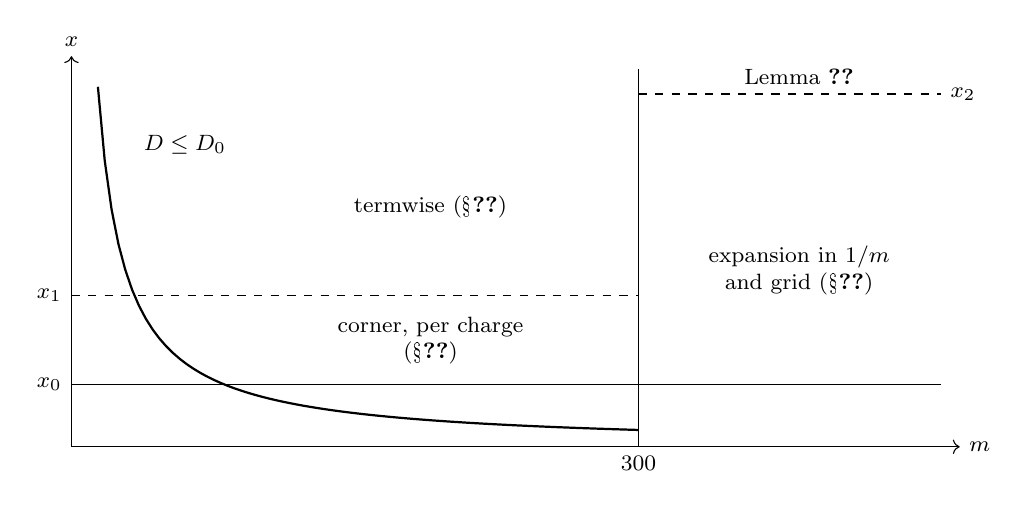
\begin{tikzpicture}[x=0.024cm,y=3.2cm,font=\footnotesize]
\draw[->] (0,0) -- (470,0) node[right] {$m$};
\draw[->] (0,0) -- (0,1.55) node[above] {$x$};
\draw (0,0.247) -- (460,0.247); \node[left] at (0,0.247) {$x_0$};
\draw[dashed] (0,0.6) -- (300,0.6); \node[left] at (0,0.6) {$x_1$};
\draw[dashed] (300,1.4) -- (460,1.4); \node[right] at (460,1.4) {$x_2$};
\draw (300,0) -- (300,1.5); \node[below] at (300,0) {$300$};
\draw[domain=14:300,samples=80,thick] plot (\x,{min(1.5,20/\x)});
\node at (60,1.2) {$D\le D_0$};
\node[align=center] at (190,0.42) {corner, per charge\\ (\S\ref{sec:corner})};
\node[align=center] at (190,0.95) {termwise (\S\ref{sec:away})};
\node[align=center] at (385,0.7) {expansion in $1/m$\\ and grid (\S\ref{sec:large})};
\node[align=center] at (385,1.47) {Lemma~\ref{lem:largex}};
\end{tikzpicture}
\caption{The regions of the proof for $N=7$, in the plane of $m=\frac N2Q^2$ and $x=\sqrt D/m$; the curve is $D=D_0$. Reduced charges lie above $x=x_0$. The pictures for $N=3,5$ are the same with the constants of Tables~\ref{tab:Pmin} and \ref{tab:corner}.}
\label{fig:regions}
\end{figure}

%%==================================================================
\section{Checks and Remarks}\label{sec:checks}
%%==================================================================

The smallest values of $\cL$ in the corner, $0.2057$, $0.1993$ and $0.1651$, are close to the minima of $|P_N|^2$ in Table~\ref{tab:Pmin}; the minimum is attained near $\ell=m$ (for $N=3,5$) and near $\ell/m\approx0.71$ (for $N=7$), on the lower boundary $x=x_0$ of the reduced region, which is where the cancellation inside $|P_N(z)|^2$ is strongest. The margin of the large-$m$ grid is smallest in the first cell above $x_0$, and the remainders $E_1,E_2$ there are below $0.04$.

For $N=2$ the same method gives the result of \cite{Bha26a} with the constant $0.5389$ in place of Table~\ref{tab:Pmin}; the higher-order expansion of Section~\ref{sec:large} was not needed there because the minimum of $|P_2|^2$ is large enough for termwise bounds.

\subsection*{Data availability}
The Python programs for every computation in this paper (the exact expansion of the product formula, the checks of Proposition~\ref{prop:walls} and Theorem~\ref{thm:exp}, the error bounds, the corner and grid certifications, and the figures) are available in the GitHub repository \url{https://github.com/anaxia-research/chl-positivity}, together with the source of this article and the output logs.

\subsection*{Funding}
This research received no external funding.

\subsection*{Conflicts of interest}
The author declares no conflicts of interest.

\begin{thebibliography}{99}
\bibitem{Sen11} A. Sen, \emph{How do black holes predict the sign of the Fourier coefficients of Siegel modular forms?}, Gen. Relativ. Gravit. \textbf{43} (2011), 2171--2183. \href{https://doi.org/10.1007/s10714-011-1175-9}{doi:10.1007/s10714-011-1175-9}
\bibitem{Sen08} A. Sen, \emph{Black hole entropy function, attractors and precision counting of microstates}, Gen. Relativ. Gravit. \textbf{40} (2008), 2249--2431. \href{https://doi.org/10.1007/s10714-008-0626-4}{doi:10.1007/s10714-008-0626-4}
\bibitem{DVV97} R. Dijkgraaf, E. Verlinde, H. Verlinde, \emph{Counting dyons in $\mathcal N=4$ string theory}, Nucl. Phys. B \textbf{484} (1997), 543--561. \href{https://doi.org/10.1016/S0550-3213(96)00640-2}{doi:10.1016/S0550-3213(96)00640-2}
\bibitem{BM13} K. Bringmann, S. Murthy, \emph{On the positivity of black hole degeneracies in string theory}, Commun. Number Theory Phys. \textbf{7} (2013), 15--56. \href{https://doi.org/10.4310/CNTP.2013.v7.n1.a2}{doi:10.4310/CNTP.2013.v7.n1.a2}
\bibitem{Ros24} M. Rossell\'o, \emph{The immortal dyon index is positive}, preprint (2024). \href{https://arxiv.org/abs/2403.19630}{arXiv:2403.19630}
\bibitem{CHL95} S. Chaudhuri, G. Hockney, J. D. Lykken, \emph{Maximally supersymmetric string theories in $D<10$}, Phys. Rev. Lett. \textbf{75} (1995), 2264--2267. \href{https://doi.org/10.1103/PhysRevLett.75.2264}{doi:10.1103/PhysRevLett.75.2264}
\bibitem{JS06} D. P. Jatkar, A. Sen, \emph{Dyon spectrum in CHL models}, J. High Energy Phys. 2006, no.~4 (2006), 018. \href{https://doi.org/10.1088/1126-6708/2006/04/018}{doi:10.1088/1126-6708/2006/04/018}
\bibitem{DJS06} J. R. David, D. P. Jatkar, A. Sen, \emph{Product representation of dyon partition function in CHL models}, J. High Energy Phys. 2006, no.~6 (2006), 064. \href{https://doi.org/10.1088/1126-6708/2006/06/064}{doi:10.1088/1126-6708/2006/06/064}
\bibitem{BSS25} A. Bhand, A. Sen, R. K. Singh, \emph{Mock modularity in CHL models}, Res. Math. Sci. \textbf{12} (2025), 8. \href{https://doi.org/10.1007/s40687-024-00489-0}{doi:10.1007/s40687-024-00489-0}
\bibitem{Bha26a} D. Bhattacharjee, \emph{Every single-centred black hole index of the $\mathbb Z_2$ CHL model is positive}, Preprints (2026), version~2. \href{https://doi.org/10.20944/preprints202611.1118.v2}{doi:10.20944/preprints202611.1118.v2}
\bibitem{Bha26b} D. Bhattacharjee, \emph{Positive black hole indices in $\mathcal N=4$ and $\mathcal N=8$ string theory}, Preprints (2026), version~2. \href{https://doi.org/10.20944/preprints202611.1219.v2}{doi:10.20944/preprints202611.1219.v2}
\bibitem{EZ85} M. Eichler, D. Zagier, \emph{The Theory of Jacobi Forms}, Progress in Mathematics 55, Birkh\"auser, Boston, 1985. \href{https://doi.org/10.1007/978-1-4684-9162-3}{doi:10.1007/978-1-4684-9162-3}
\bibitem{DMZ12} A. Dabholkar, S. Murthy, D. Zagier, \emph{Quantum black holes, wall crossing and mock modular forms}, preprint (2012). \href{https://arxiv.org/abs/1208.4074}{arXiv:1208.4074}
\bibitem{Bha26c} D. Bhattacharjee, \emph{Positive first-row black hole indices in CHL models}, preprint (2026).
\bibitem{Sin26} R. K. Singh, \emph{Generating function of single-centered black hole index in CHL models}, preprint (2026). \href{https://arxiv.org/abs/2606.19479}{arXiv:2606.19479}
\bibitem{BM13a} K. Bringmann, J. Manschot, \emph{From sheaves on $\mathbb P^2$ to a generalization of the Rademacher expansion}, Amer. J. Math. \textbf{135} (2013), 1039--1065. \href{https://doi.org/10.1353/ajm.2013.0031}{doi:10.1353/ajm.2013.0031}
\bibitem{FR17} A. Ferrari, V. Reys, \emph{Mixed Rademacher and BPS black holes}, J. High Energy Phys. 2017, no.~7 (2017), 094. \href{https://doi.org/10.1007/JHEP07(2017)094}{doi:10.1007/JHEP07(2017)094}
\bibitem{CNR21} G. L. Cardoso, S. Nampuri, M. Rossell\'o, \emph{Arithmetic of decay walls through continued fractions: a new exact dyon counting solution in $\mathcal N=4$ CHL models}, J. High Energy Phys. 2021, no.~3 (2021), 154. \href{https://doi.org/10.1007/JHEP03(2021)154}{doi:10.1007/JHEP03(2021)154}
\bibitem{CKMRW20} A. Chowdhury, A. Kidambi, S. Murthy, V. Reys, T. Wrase, \emph{Dyonic black hole degeneracies in $\mathcal N=4$ string theory from Dabholkar--Harvey degeneracies}, J. High Energy Phys. 2020, no.~10 (2020), 184. \href{https://doi.org/10.1007/JHEP10(2020)184}{doi:10.1007/JHEP10(2020)184}
\bibitem{Bor98} R. E. Borcherds, \emph{Automorphic forms with singularities on Grassmannians}, Invent. Math. \textbf{132} (1998), 491--562. \href{https://doi.org/10.1007/s002220050232}{doi:10.1007/s002220050232}
\bibitem{Son65} R. P. Soni, \emph{On an inequality for modified Bessel functions}, J. Math. Phys. \textbf{44} (1965), 406--407. \href{https://doi.org/10.1002/sapm1965441406}{doi:10.1002/sapm1965441406}
\bibitem{Joh17} F. Johansson, \emph{Arb: efficient arbitrary-precision midpoint-radius interval arithmetic}, IEEE Trans. Comput. \textbf{66} (2017), 1281--1292. \href{https://doi.org/10.1109/TC.2017.2690633}{doi:10.1109/TC.2017.2690633}
\bibitem{DLMF} F. W. J. Olver, A. B. Olde Daalhuis, D. W. Lozier, B. I. Schneider, R. F. Boisvert, C. W. Clark, B. R. Miller, B. V. Saunders, H. S. Cohl, M. A. McClain (eds.), \emph{NIST Digital Library of Mathematical Functions}, Chapter~10. \url{https://dlmf.nist.gov/10}
\end{thebibliography}
\end{document}
